%%  ************    LibreSilicon's 1st TestWafer    *******************
%%
%%  Organisation:   Chipforge
%%                  Germany / European Union
%%
%%  Profile:        Chipforge focus on fine System-on-Chip Cores in
%%                  Verilog HDL Code which are easy understandable and
%%                  adjustable. For further information see
%%                          www.chipforge.org
%%                  there are projects from small cores up to PCBs, too.
%%
%%  File:           PearlRiver/Documents/LaTeX/pearlriver.tex
%%
%%  Purpose:        Top Level File for 1st Test Wafer Documentation
%%
%%  ************    LuaLaTeX with circdia.sty package   ***************
%%
%%  ///////////////////////////////////////////////////////////////////
%%
%%  Copyright (c) 2018 by chipforge <hsank@nospam.chipforge.org>
%%  All rights reserved.
%%
%%      This Standard Cell Library is licensed under the Libre Silicon
%%      public license; you can redistribute it and/or modify it under
%%      the terms of the Libre Silicon public license as published by
%%      the Libre Silicon alliance, either version 1 of the License, or
%%      (at your option) any later version.
%%
%%      This design is distributed in the hope that it will be useful,
%%      but WITHOUT ANY WARRANTY; without even the implied warranty of
%%      MERCHANTABILITY or FITNESS FOR A PARTICULAR PURPOSE.
%%      See the Libre Silicon Public License for more details.
%%
%%  ///////////////////////////////////////////////////////////////////
\documentclass[a4paper,english,twoside]{article}
\usepackage{fontspec}
\usepackage{amssymb}
\usepackage{mathtools}
\usepackage{babel}
\usepackage{luatexja-fontspec}
\usepackage[digital,srcmeas,semicon]{circdia}
\usepackage[left=2cm,right=2cm,top=1.5cm,bottom=3cm]{geometry}

\defaultfontfeatures{Ligatures=TeX}
%\setmainfont{Linux Libertine 0}
\setmainjfont{FandolSong}
%\setsansfont{Kurier}
%\setsansfont{Menlo}

\title{PearlRiver -- LibreSilicon's 1st Test Wafer (珠江芯片一号)}
\author{Hagen Sankowski}
\date{\today}

\makeindex  % usefull for ToC
\setlength{\parindent}{0em} % get rid of annoying indents
\setlength{\parskip}{0.5em}

\begin{document}
\maketitle

\begin{abstract}
\begin{quote}
Copyright \textcopyright  2018 CHIPFORGE.ORG. All rights reserved. \\

This process is licensed under the Libre Silicon public license; you can redistribute it and/or modify it under the terms of the Libre Silicon public license as published by the Libre Silicon alliance either version 1 of the License, or (at your option) any later version. \\

This design is distributed in the hope that it will be useful, but \textsc{WITHOUT ANY WARRANTY}; without even the implied warranty of \textsc{MERCHANTABILITY} or \textsc{FITNESS FOR A PARTICULAR PURPOSE}. See the Libre Silicon Public License for more details. \\

For further clarification consult the complete documentation of the process.
\end{quote}
\end{abstract}
\clearpage
%%  ************    LibreSilicon's 1st TestWafer    *******************
%%
%%  Organisation:   Chipforge
%%                  Germany / European Union
%%
%%  Profile:        Chipforge focus on fine System-on-Chip Cores in
%%                  Verilog HDL Code which are easy understandable and
%%                  adjustable. For further information see
%%                          www.chipforge.org
%%                  there are projects from small cores up to PCBs, too.
%%
%%  File:           PearlRiver/Documents/LaTeX/revision.tex
%%
%%  Purpose:        Revision History File
%%
%%  ************    LaTeX with circdia.sty package      ***************
%%
%%  ///////////////////////////////////////////////////////////////////
%%
%%  Copyright (c) 2018 by chipforge <hsank@nospam.chipforge.org>
%%  All rights reserved.
%%
%%      This Standard Cell Library is licensed under the Libre Silicon
%%      public license; you can redistribute it and/or modify it under
%%      the terms of the Libre Silicon public license as published by
%%      the Libre Silicon alliance, either version 1 of the License, or
%%      (at your option) any later version.
%%
%%      This design is distributed in the hope that it will be useful,
%%      but WITHOUT ANY WARRANTY; without even the implied warranty of
%%      MERCHANTABILITY or FITNESS FOR A PARTICULAR PURPOSE.
%%      See the Libre Silicon Public License for more details.
%%
%%  ///////////////////////////////////////////////////////////////////
Document Revision History
\begin{table}[h] %\caption{Document Revision History}
    \begin{tabular}{|l|c|ll|} \hline
        VERSION & DATE & DESCRIPTION & TRACKING NOTES\\ \hline\hline
        Draft 0.0 & 2018-05-25 & START with empty document, ADD Ring Oscillator & -\\ \hline
    \end{tabular}
\end{table}


PearlRiver is the first Test Wafer for the LibreSilicon 1 $ \mu m$ Technology.

This Testwafer contains almost all test structures to evaulate and qualify the technology-depended parameters.
On Wafer are placed structures to measure the sheet-resistance of all Poly and Metal Layer, as well Capacitors, NMOS and PMOS Transistors, Bipolar Junction Transistors, Diodes and Flash cells.
There are even common cells like NANDs, NORs and Inverters forming ring oscillators.

All parameters, measured from all test structures are used for Spice3f simulation models.

\clearpage
\tableofcontents
\clearpage

\pagestyle{headings}
\renewcommand{\theequation}{\thesection.\arabic{equation}}
\numberwithin{equation}{section}

%%  ************    LibreSilicon's 1st TestWafer    *******************
%%
%%  Organisation:   Chipforge
%%                  Germany / European Union
%%
%%  Profile:        Chipforge focus on fine System-on-Chip Cores in
%%                  Verilog HDL Code which are easy understandable and
%%                  adjustable. For further information see
%%                          www.chipforge.org
%%                  there are projects from small cores up to PCBs, too.
%%
%%  File:           PearlRiver/Documents/LaTeX/considerations.tex
%%
%%  Purpose:        Chapter File for Considerations
%%
%%  ************    LaTeX with circdia.sty package      ***************
%%
%%  ///////////////////////////////////////////////////////////////////
%%
%%  Copyright (c) 2018 by chipforge <hsank@nospam.chipforge.org>
%%  All rights reserved.
%%
%%      This Standard Cell Library is licensed under the Libre Silicon
%%      public license; you can redistribute it and/or modify it under
%%      the terms of the Libre Silicon public license as published by
%%      the Libre Silicon alliance, either version 1 of the License, or
%%      (at your option) any later version.
%%
%%      This design is distributed in the hope that it will be useful,
%%      but WITHOUT ANY WARRANTY; without even the implied warranty of
%%      MERCHANTABILITY or FITNESS FOR A PARTICULAR PURPOSE.
%%      See the Libre Silicon Public License for more details.
%%
%%  ///////////////////////////////////////////////////////////////////
\section{Considerations}

\subsection{Orientation}

There are two different systems to give orientation while talking about locations on the die.
One system use words like Top (= upper side), Right, Bottom (= lower side) and Left.
The other system uses cardinal directions like North, East, South and West to name the same.
Both systems are very common, here the cardinal directions are prefered, just as convention.

%%  ************    LibreSilicon's 1st TestWafer    *******************
%%
%%  Organisation:   Chipforge
%%                  Germany / European Union
%%
%%  Profile:        Chipforge focus on fine System-on-Chip Cores in
%%                  Verilog HDL Code which are easy understandable and
%%                  adjustable. For further information see
%%                          www.chipforge.org
%%                  there are projects from small cores up to PCBs, too.
%%
%%  File:           PearlRiver/Documents/LaTeX/picture_wafer_size.tex
%%
%%  Purpose:        Picture for Wafer Size compare and Flats
%%
%%  ************    LaTeX with circdia.sty package      ***************
%%
%%  ///////////////////////////////////////////////////////////////////
%%
%%  Copyright (c) 2018 by chipforge <hsank@nospam.chipforge.org>
%%  All rights reserved.
%%
%%      This Standard Cell Library is licensed under the Libre Silicon
%%      public license; you can redistribute it and/or modify it under
%%      the terms of the Libre Silicon public license as published by
%%      the Libre Silicon alliance, either version 1 of the License, or
%%      (at your option) any later version.
%%
%%      This design is distributed in the hope that it will be useful,
%%      but WITHOUT ANY WARRANTY; without even the implied warranty of
%%      MERCHANTABILITY or FITNESS FOR A PARTICULAR PURPOSE.
%%      See the Libre Silicon Public License for more details.
%%
%%  ///////////////////////////////////////////////////////////////////
\begin{center}
    Picture - Wafer Size and Flats
    \begin{figure}[h]
        \begin{center}
            \begin{tikzpicture}[]
            \draw (0,0) arc (-60:240:5);
            \draw (0,0) arc (-60:240:6.12);
            \draw (0,0) arc (-60:240:7.5);
            \draw (0,0) -- (-7.5,0);
            \node at (-2,8) {4-inch Wafer};
            \node at (-2.5,10.5) {5-inch Wafer};
            \node at (-3,13) {6-inch Wafer};
            \node at (-3.5,-0.5) {flats on South};
            \end{tikzpicture}
        \end{center}
    \end{figure}
\end{center}


Wafers smaller than 8 inches, or 200 mm, have a flat side to give orientation and encode the crystal structure (eg. \{100\}).
In this document, the South side is the one with the flat.

\subsection{Process Variation}

All machines in the process flow affects the quality of wafer processing.
This results in Variations, regarding the location of the test structure on the wafer as well as the structures itself.

For instance etching is slightly more aggressiv on one side of a structure than on the opposite side.
One aim of the Test Wafer is also to understand und measure this effects.

Therefor the wafer is divided into many small, repetative pieces, called dies, to get quantified values for the location.
It is possible to measure structures always at the same die location over and over for many wafers.

Also, every die itself is build from four triangles (representing one side) of the same test structures to measure how the process works from different directions.
This means, that all structures are grouped together in four triangles, each rotated by 90 degrees, forming a square.

%%  ************    LibreSilicon's 1st TestWafer    *******************
%%
%%  Organisation:   Chipforge
%%                  Germany / European Union
%%
%%  Profile:        Chipforge focus on fine System-on-Chip Cores in
%%                  Verilog HDL Code which are easy understandable and
%%                  adjustable. For further information see
%%                          www.chipforge.org
%%                  there are projects from small cores up to PCBs, too.
%%
%%  File:           PearlRiver/Documents/LaTeX/die_quarter.tex
%%
%%  Purpose:        Principle Description Pictgure for quarters
%%
%%  ************    LaTeX with circdia.sty package      ***************
%%
%%  ///////////////////////////////////////////////////////////////////
%%
%%  Copyright (c) 2018 by chipforge <hsank@nospam.chipforge.org>
%%  All rights reserved.
%%
%%      This Standard Cell Library is licensed under the Libre Silicon
%%      public license; you can redistribute it and/or modify it under
%%      the terms of the Libre Silicon public license as published by
%%      the Libre Silicon alliance, either version 1 of the License, or
%%      (at your option) any later version.
%%
%%      This design is distributed in the hope that it will be useful,
%%      but WITHOUT ANY WARRANTY; without even the implied warranty of
%%      MERCHANTABILITY or FITNESS FOR A PARTICULAR PURPOSE.
%%      See the Libre Silicon Public License for more details.
%%
%%  ///////////////////////////////////////////////////////////////////
\begin{center}
    Principle - One Die with all Quarters
    \begin{figure}[h]
        \begin{center}
            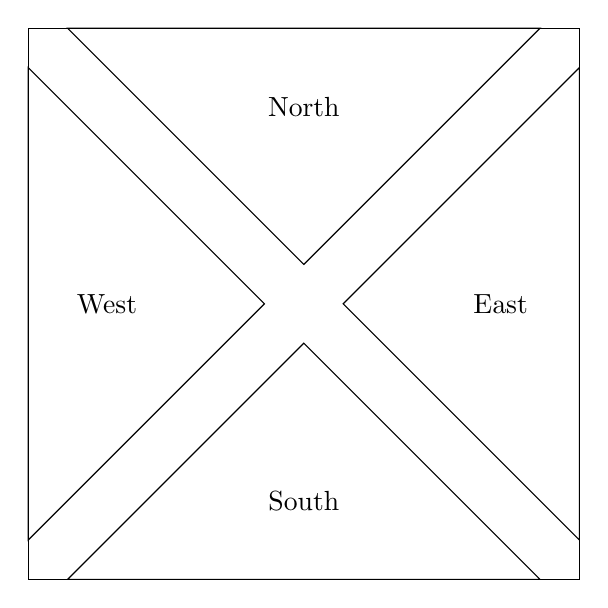
\begin{tikzpicture}[]
            \draw (0,0) -- (7,0) -- (7,7) -- (0,7) -- cycle;
            \draw (0.5,0) -- (6.5,0) -- (3.5,3) -- cycle;
            \draw (7,0.5) -- (7,6.5) -- (4,3.5) -- cycle;
            \draw (6.5,7) -- (0.5,7) -- (3.5,4) -- cycle;
            \draw (0,6.5) -- (0,0.5) -- (3,3.5) -- cycle;
            \node at (6,3.5) {East};
            \node at (3.5,6) {North};
            \node at (1,3.5) {West};
            \node at (3.5,1) {South};
            \end{tikzpicture}
        \end{center}
    \end{figure}
\end{center}


Quantifying the test structures, the location can be referenced by the die position and the quarter (North, East, South and West) on die where the test structures is measured.
There is no recommandations about the metrics for the location.

\subsection{Four-terminal Sensing}

The prefered measurement method for the test structures is the so-calld Four-terminal Sensing, or Kelvin sensing.
This is an electrical impedance measuring technique that uses pairs of current-carrying and voltage-sensing probes to make accurate measurements.

Four-terminal Sensing has advantage for precise measurement of low resistance values by eliminationg the lead and contact resistance for the measurement.
Therefor almost all test structures here using four contact pads to place the probes on them.

%%  ************    LibreSilicon's 1st TestWafer    *******************
%%
%%  Organisation:   Chipforge
%%                  Germany / European Union
%%
%%  Profile:        Chipforge focus on fine System-on-Chip Cores in
%%                  Verilog HDL Code which are easy understandable and
%%                  adjustable. For further information see
%%                          www.chipforge.org
%%                  there are projects from small cores up to PCBs, too.
%%
%%  File:           PearlRiver/Documents/LaTeX/schematic_4terminal.tex
%%
%%  Purpose:        Schematic File for Four-terminal Sensing
%%
%%  ************    LaTeX with circdia.sty package      ***************
%%
%%  ///////////////////////////////////////////////////////////////////
%%
%%  Copyright (c) 2018 by chipforge <hsank@nospam.chipforge.org>
%%  All rights reserved.
%%
%%      This Standard Cell Library is licensed under the Libre Silicon
%%      public license; you can redistribute it and/or modify it under
%%      the terms of the Libre Silicon public license as published by
%%      the Libre Silicon alliance, either version 1 of the License, or
%%      (at your option) any later version.
%%
%%      This design is distributed in the hope that it will be useful,
%%      but WITHOUT ANY WARRANTY; without even the implied warranty of
%%      MERCHANTABILITY or FITNESS FOR A PARTICULAR PURPOSE.
%%      See the Libre Silicon Public License for more details.
%%
%%  ///////////////////////////////////////////////////////////////////
\begin{center}
    Four-terminal Sensing with instrument, probes and device-under-test
    \begin{figure}[h]
        \begin{center}
            \begin{circuitdiagram}{42}{25}
            % current source with ground
            \ground{3}{0}{D}
            \wire{3}{1}{3}{8}
            \othersrc[\modify{RU}]{oo}{3}{11}{V}{}{}
            \wire{3}{14}{3}{21}
            % vertical flow, ampere meter
            \wire{3}{21}{12}{21}
            \measdev[\measunit{A}]{15}{21}{H}{$I_{drive}$}{}
            \wire{18}{21}{24}{21}
            \currarrow{20}{21}{R}{I}
            % pin contact
            \pin[\female]{25}{21}{R}{}
            \pin[\male]{25}{21}{L}{}
            %
            \pin[\female]{25}{1}{R}{}
            \pin[\male]{25}{1}{L}{}
            \ground{24}{0}{D}
            %
            \pin[\female]{25}{6}{R}{}
            \pin[\male]{25}{6}{L}{}
            %
            \pin[\female]{25}{16}{R}{}
            \pin[\male]{25}{16}{L}{}
            % voltage measurement
            \wire{15}{14}{15}{16}
            \wire{15}{16}{24}{16}
            \measdev[\measunit{V}]{15}{11}{V}{$V_{meas}$}{}
            \wire{15}{6}{15}{8}
            \wire{15}{6}{24}{6}
            \Voltarrow{25}{16}{25}{6}{r}{U}
            % device under test
            \resis{40}{11}{V}{DUT}{}
            \wire{26}{1}{35.5}{1}
            \pin{40}{1}{Dr}{}
            \power{35}{1}{R}{I-}
            \wire{26}{6}{35.5}{6}
            \pin{40}{6}{UD}{}
            \power{35}{6}{R}{U-}
            \wire{26}{16}{35.5}{16}
            \pin{40}{16}{UD}{}
            \power{35}{16}{R}{U+}
            \wire{26}{21}{35.5}{21}
            \pin{40}{21}{Ur}{}
            \power{35}{21}{R}{I+}
            %
            \wire{40}{2}{40}{5}
            \wire{40}{7}{40}{8}
            \wire{40}{14}{40}{15}
            \wire{40}{17}{40}{20}
            \end{circuitdiagram}
        \end{center}
    \end{figure}
\end{center}


Best results are given, when the sense wire probes are placed close to device-under-test (DUT) as the inside pair, while the force wire probes are the outside pair.
Otherwise the accuracy can be affected, because more of the lead is included in the measurement.

It is also recommended that every measurement starts with very low current, while voltages could break the test structures.
The current respects the total resistance on the path and results in a voltage which can be measured on the sensing wire probes.
Regarding Ohm's law

\begin{equation}\label{1}
    Resistance = \frac{Voltage}{Current}
\end{equation}

the Resistance can be calculated by driven Current and resulting Voltage.


%%  ************    LibreSilicon's 1st TestWafer    *******************
%%
%%  Organisation:   Chipforge
%%                  Germany / European Union
%%
%%  Profile:        Chipforge focus on fine System-on-Chip Cores in
%%                  Verilog HDL Code which are easy understandable and
%%                  adjustable. For further information see
%%                          www.chipforge.org
%%                  there are projects from small cores up to PCBs, too.
%%
%%  File:           PearlRiver/Documents/LaTeX/die_quarter.tex
%%
%%  Purpose:        Principle Description Pictgure for quarters
%%
%%  ************    LaTeX with circdia.sty package      ***************
%%
%%  ///////////////////////////////////////////////////////////////////
%%
%%  Copyright (c) 2018 by chipforge <hsank@nospam.chipforge.org>
%%  All rights reserved.
%%
%%      This Standard Cell Library is licensed under the Libre Silicon
%%      public license; you can redistribute it and/or modify it under
%%      the terms of the Libre Silicon public license as published by
%%      the Libre Silicon alliance, either version 1 of the License, or
%%      (at your option) any later version.
%%
%%      This design is distributed in the hope that it will be useful,
%%      but WITHOUT ANY WARRANTY; without even the implied warranty of
%%      MERCHANTABILITY or FITNESS FOR A PARTICULAR PURPOSE.
%%      See the Libre Silicon Public License for more details.
%%
%%  ///////////////////////////////////////////////////////////////////
\begin{center}
    Principle - $R_\square$
    \begin{figure}[h]
        \begin{center}
            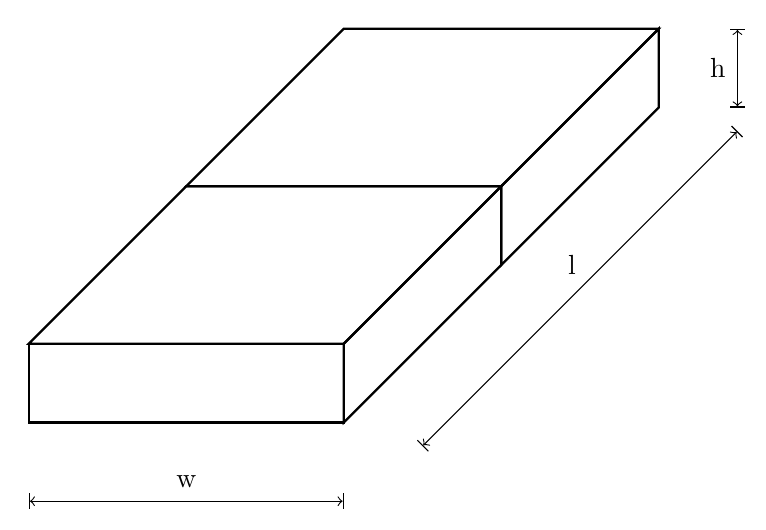
\begin{tikzpicture}[]
            \draw[thick] (0,0) -- (4,0) -- (4,1) -- (0,1) -- cycle; % front
            \draw[thick] (0,1) -- (2,3) -- (6,3) -- (4,1) -- cycle; % 1st top
            \draw[thick] (4,0) -- (4,1) -- (6,3) -- (6,2) -- cycle; % 1st boarder
            \draw[thick] (2,3) -- (4,5) -- (8,5) -- (6,3) -- cycle; % 2nd top
            \draw[thick] (6,3) -- (8,5) -- (8,4) -- (6,2) -- cycle; % 2nd boarder
            % width
            \node at (2,-0.75) {w};
            \draw[|<->|] (0,-1) -- (4,-1);
            % length
            \node at (6.9,2) {l};
            \draw[|<->|] (5,-0.3) -- (9,3.7);
            % hight
            \node at (8.75,4.5) {h};
            \draw[|<->|] (9,4) -- (9,5);
            \end{tikzpicture}
        \end{center}
    \end{figure}
\end{center}


\clearpage

%%  ************    LibreSilicon's 1st TestWafer    *******************
%%
%%  Organisation:   Chipforge
%%                  Germany / European Union
%%
%%  Profile:        Chipforge focus on fine System-on-Chip Cores in
%%                  Verilog HDL Code which are easy understandable and
%%                  adjustable. For further information see
%%                          www.chipforge.org
%%                  there are projects from small cores up to PCBs, too.
%%
%%  File:           PearlRiver/Documents/LaTeX/ringoscillators.tex
%%
%%  Purpose:        Chapter File for Ring Oscillators
%%
%%  ************    LaTeX with circdia.sty package      ***************
%%
%%  ///////////////////////////////////////////////////////////////////
%%
%%  Copyright (c) 2018 by chipforge <hsank@nospam.chipforge.org>
%%  All rights reserved.
%%
%%      This Standard Cell Library is licensed under the Libre Silicon
%%      public license; you can redistribute it and/or modify it under
%%      the terms of the Libre Silicon public license as published by
%%      the Libre Silicon alliance, either version 1 of the License, or
%%      (at your option) any later version.
%%
%%      This design is distributed in the hope that it will be useful,
%%      but WITHOUT ANY WARRANTY; without even the implied warranty of
%%      MERCHANTABILITY or FITNESS FOR A PARTICULAR PURPOSE.
%%      See the Libre Silicon Public License for more details.
%%
%%  ///////////////////////////////////////////////////////////////////
\section{Ring Oscillators}

Ring Oscillators are the hidden Champions in case of qualifying a process.

Here is a example of a Ring Oscillator with 5 inverting stages (build with inverters).

%%  ************    LibreSilicon's 1st TestWafer    *******************
%%
%%  Organisation:   Chipforge
%%                  Germany / European Union
%%
%%  Profile:        Chipforge focus on fine System-on-Chip Cores in
%%                  Verilog HDL Code which are easy understandable and
%%                  adjustable. For further information see
%%                          www.chipforge.org
%%                  there are projects from small cores up to PCBs, too.
%%
%%  File:           PearlRiver/Documents/LaTeX/schematic_invring.tex
%%
%%  Purpose:        Schematic File for Ring Oscillator with INV-Gates
%%
%%  ************    LaTeX with circdia.sty package      ***************
%%
%%  ///////////////////////////////////////////////////////////////////
%%
%%  Copyright (c) 2018 by chipforge <hsank@nospam.chipforge.org>
%%  All rights reserved.
%%
%%      This Standard Cell Library is licensed under the Libre Silicon
%%      public license; you can redistribute it and/or modify it under
%%      the terms of the Libre Silicon public license as published by
%%      the Libre Silicon alliance, either version 1 of the License, or
%%      (at your option) any later version.
%%
%%      This design is distributed in the hope that it will be useful,
%%      but WITHOUT ANY WARRANTY; without even the implied warranty of
%%      MERCHANTABILITY or FITNESS FOR A PARTICULAR PURPOSE.
%%      See the Libre Silicon Public License for more details.
%%
%%  ///////////////////////////////////////////////////////////////////
\begin{center}
    Schematic (Ring Oscillator with INV-Gates)
    \begin{figure}[h]
        \begin{center}
            \begin{circuitdiagram}{60}{9}
            \pin{1}{7}{L}{EN} % pin EN, enable oscillation
            \pin{59}{5}{R}{$f_{INV}$} % pin FINV,
            \gate[\inputs{2}]{nand}{5}{5}{R}{}{}    % NAND gate -> right
            \wire{9}{5}{12}{5}  % interconnect wire
            \gate{not}{15}{5}{R}{}{} % INV gate -> right
            \wire{18}{5}{22}{5}  % interconnect wire
            \gate{not}{25}{5}{R}{}{} % INV gate -> right
            \wire{28}{5}{32}{5}  % interconnect wire
            \gate{not}{35}{5}{R}{}{} % INV gate -> right
            \wire{38}{5}{42}{5}  % interconnect wire
            \gate{not}{45}{5}{R}{}{} % INV gate -> right
            \wire{48}{5}{52}{5}  % interconnect wire
            \gate{not}{55}{5}{R}{}{} % INV gate -> right
            \junct{51}{5}
            \wire{51}{5}{51}{1}     % feedback wire
            \wire{2}{1}{51}{1}  % interconnect wire
            \wire{2}{1}{2}{3}     % feedback wire
            \end{circuitdiagram}
        \end{center}
    \end{figure}
\end{center}


If $EN = 0$ the Ring Oscillator does nothing. But when $EN$ becomes $1$, the output of the most left NAND2 Gate depends on the other input. With both inputs for the NAND2 Gate are $1$, the output goes to $0$, otherwise the output is $1$.

Hence we can describe $EN$ as a high-active Enable signal.

Assuming now $EN = 1$, the Ring Oscillator is enabled, the NAND3 Gate delivers the inverted input value from the long feedback line on his output. Assuming there was a level change, this edge propagates through every gate (which takes time $t_D$ for every INV Gate). At $n \cdot t_D$ this edge cames back over the feedback line with inverted polarity, while using odd numbers only of inverting Gates.

While edges progagates once through the long line of inverting gates and arrives on the enabling gate again inverted, after 2 runs, this forms a waveform on $f_{INV}$ which is similiar to a clock with a 50-50 duty cycle. The last buffer, between the feedback line and the output pin, is just a buffer to keep the driven capacaty on the output line low.
Now we can say, that the frequency of the output signal depends just on the delay $t_D$ over the inverting gates. The Equation for odd numbers of $n$ is

\begin{equation}\label{f_inv}
    f_{INV} = \frac{1}{2n \cdot t_D}
\end{equation}

Usually, Ring Oscillators are build from 100..150 Gates in one row. The reason for that is the lowpass characteristic of PAD Cells - the output frequency on PAD cells should be below their cut-off frequency.

With a reasonable guessed value of $t_D$ and equation \ref{f_inv} we can now adjust $f_{INV}$ below the cut-off frequency.

At this point we should think about $t_D$ which depends of course from different parameters, at least

\begin{enumerate}
\item the Supply Voltage for the inverting Gates,
\item the current Temperature,
\item and the Quality of the processed technology for every Gate.
\end{enumerate}

All three items matter for Process Evaluation and Process Calibration, just by indirect measurement of $t_D$ under different test conditions. BTW, $t_D$ follows equation \ref{f_inv} as

\begin{equation}\label{t_D}
    t_D = \frac{1}{2n \cdot f_{INV}}
\end{equation}

If you are already familiar with cell design, you migth be knowing that the delay $t_D$ over the gate differs for both edges. We assume here, that the transistor sizes for PMOS and NMOS transistors are well balanced with a relationship of $\gamma = 2$ and therefor $t_D$ has the same value for both edges.

With knowledge of the Ring Oscillator build by simple Inverting Gates, we might think about more advanced cells with different transistor sizes. The schematic with NAND Gates looks quite similiar.

%%  ************    LibreSilicon's 1st TestWafer    *******************
%%
%%  Organisation:   Chipforge
%%                  Germany / European Union
%%
%%  Profile:        Chipforge focus on fine System-on-Chip Cores in
%%                  Verilog HDL Code which are easy understandable and
%%                  adjustable. For further information see
%%                          www.chipforge.org
%%                  there are projects from small cores up to PCBs, too.
%%
%%  File:           PearlRiver/Documents/LaTeX/schematic_nand3ring.tex
%%
%%  Purpose:        Schematic File for Ring Oscillator with NAND3-Gates
%%
%%  ************    LaTeX with circdia.sty package      ***************
%%
%%  ///////////////////////////////////////////////////////////////////
%%
%%  Copyright (c) 2018 by chipforge <hsank@nospam.chipforge.org>
%%  All rights reserved.
%%
%%      This Standard Cell Library is licensed under the Libre Silicon
%%      public license; you can redistribute it and/or modify it under
%%      the terms of the Libre Silicon public license as published by
%%      the Libre Silicon alliance, either version 1 of the License, or
%%      (at your option) any later version.
%%
%%      This design is distributed in the hope that it will be useful,
%%      but WITHOUT ANY WARRANTY; without even the implied warranty of
%%      MERCHANTABILITY or FITNESS FOR A PARTICULAR PURPOSE.
%%      See the Libre Silicon Public License for more details.
%%
%%  ///////////////////////////////////////////////////////////////////
\begin{center}
    Schematic (Ring Oscillator with NAND3-Gates)
    \begin{figure}[h]
        \begin{center}
            \begin{circuitdiagram}{60}{9}
            \pin{1}{7}{L}{EN} % pin EN, enable oscillation
            \pin{59}{5}{R}{$f_{NAND}$} % pin FNAND,
            \gate[\inputs{2}]{nand}{5}{5}{R}{}{}    % NAND gate -> right
            \wire{9}{5}{12}{5}  % interconnect wire
            \wire{12}{3}{12}{7} % gate shortage
            \junct{12}{5}
            \gate[\inputs{3}]{nand}{15}{5}{R}{}{} % NAND gate -> right
            \wire{19}{5}{22}{5}  % interconnect wire
            \wire{22}{3}{22}{7} % gate shortage
            \junct{22}{5}
            \gate[\inputs{3}]{nand}{25}{5}{R}{}{} % NAND gate -> right
            \wire{29}{5}{32}{5}  % interconnect wire
            \wire{32}{3}{32}{7} % gate shortage
            \junct{32}{5}
            \gate[\inputs{3}]{nand}{35}{5}{R}{}{} % NAND gate -> right
            \wire{39}{5}{42}{5}  % interconnect wire
            \wire{42}{3}{42}{7} % gate shortage
            \junct{42}{5}
            \gate[\inputs{3}]{nand}{45}{5}{R}{}{} % NAND gate -> right
            \wire{49}{5}{52}{5}  % interconnect wire
            \gate{not}{55}{5}{R}{}{} % INV gate -> right
            \junct{51}{5}
            \wire{51}{5}{51}{1}     % feedback wire
            \wire{2}{1}{51}{1}  % interconnect wire
            \wire{2}{1}{2}{3}     % feedback wire
            \end{circuitdiagram}
        \end{center}
    \end{figure}
\end{center}


While using 3-input NAND Gates, all inputs on every gate are wired together. Using just 2-input NAND Gates would be possible also but not recommended as 3-input NAND Gates having one more stacked transisor and are heavier to process accuratly. Hence getting the oscillating output frequency on $f_{NAND}$ means much more.

Adapting the same scheme on NOR3-Gates we get this third Ring Oscillator schematic.

%%  ************    LibreSilicon's 1st TestWafer    *******************
%%
%%  Organisation:   Chipforge
%%                  Germany / European Union
%%
%%  Profile:        Chipforge focus on fine System-on-Chip Cores in
%%                  Verilog HDL Code which are easy understandable and
%%                  adjustable. For further information see
%%                          www.chipforge.org
%%                  there are projects from small cores up to PCBs, too.
%%
%%  File:           PearlRiver/Documents/LaTeX/schematic_nor3ring.tex
%%
%%  Purpose:        Schematic File for Ring Oscillator with NOR3-Gates
%%
%%  ************    LaTeX with circdia.sty package      ***************
%%
%%  ///////////////////////////////////////////////////////////////////
%%
%%  Copyright (c) 2018 by chipforge <hsank@nospam.chipforge.org>
%%  All rights reserved.
%%
%%      This Standard Cell Library is licensed under the Libre Silicon
%%      public license; you can redistribute it and/or modify it under
%%      the terms of the Libre Silicon public license as published by
%%      the Libre Silicon alliance, either version 1 of the License, or
%%      (at your option) any later version.
%%
%%      This design is distributed in the hope that it will be useful,
%%      but WITHOUT ANY WARRANTY; without even the implied warranty of
%%      MERCHANTABILITY or FITNESS FOR A PARTICULAR PURPOSE.
%%      See the Libre Silicon Public License for more details.
%%
%%  ///////////////////////////////////////////////////////////////////
\begin{center}
    Schematic (Ring Oscillator with NOR3-Gates)
    \begin{figure}[h]
        \begin{center}
            \begin{circuitdiagram}{60}{9}
            \pin{1}{7}{L}{$\overline{EN}$} % pin EN, enable oscillation
            \pin{59}{5}{R}{$f_{NOR}$} % pin FNOR,
            \gate[\inputs{2}]{nor}{5}{5}{R}{}{}    % NOR gate -> right
            \wire{9}{5}{12}{5}  % interconnect wire
            \wire{12}{3}{12}{7} % gate shortage
            \junct{12}{5}
            \gate[\inputs{3}]{nor}{15}{5}{R}{}{} % NOR gate -> right
            \wire{19}{5}{22}{5}  % interconnect wire
            \wire{22}{3}{22}{7} % gate shortage
            \junct{22}{5}
            \gate[\inputs{3}]{nor}{25}{5}{R}{}{} % NOR gate -> right
            \wire{29}{5}{32}{5}  % interconnect wire
            \wire{32}{3}{32}{7} % gate shortage
            \junct{32}{5}
            \gate[\inputs{3}]{nor}{35}{5}{R}{}{} % NOR gate -> right
            \wire{39}{5}{42}{5}  % interconnect wire
            \wire{42}{3}{42}{7} % gate shortage
            \junct{42}{5}
            \gate[\inputs{3}]{nor}{45}{5}{R}{}{} % NOR gate -> right
            \wire{49}{5}{52}{5}  % interconnect wire
            \gate{not}{55}{5}{R}{}{} % INV gate -> right
            \junct{51}{5}
            \wire{51}{5}{51}{1}     % feedback wire
            \wire{2}{1}{51}{1}  % interconnect wire
            \wire{2}{1}{2}{3}     % feedback wire
            \end{circuitdiagram}
        \end{center}
    \end{figure}
\end{center}


Now please, make yourself familiar with the method of "Logical Effort" for calculating the transistor sizes to get well balanced cells. We still assume that $\gamma = 2$, where the PMOS transistors are 2 times bigger than the NMOS transistors.

As the logical effort differs for every type of Gate (and therefor there delay), we can calculate the relationship between all output frequencies $f_{INV}$, $f_{NAND}$ and $f_{NOR}$.

The highest output frequency should have the INV Gate based Ring Oscillator ($f_{INV}$) with the lowest logical effort $g = \frac{3}{3}$, followed by the NAND3 Gate based Ring Oscillator ($f_{NAND}$) with logical effort $g = \frac{5}{3}$. The lowest frequency should have the NOR3 Gate based Ring Oscillator ($f_{NOR}$) with logical effort of $g = \frac{7}{3}$.

According the calculation of getting the delay from the logical effort, the relations can be expressed as
%
\begin{equation}
    f_{INV} \approx f_{max}
\end{equation}
%
\begin{equation}
    f_{NAND} \approx \frac{9}{11} \cdot f_{INV}
\end{equation}
%
\begin{equation}
    f_{NOR} \approx \frac{9}{13} \cdot f_{INV}
\end{equation}

\clearpage


%%  ************    LibreSilicon's 1st TestWafer    *******************
%%
%%  Organisation:   Chipforge
%%                  Germany / European Union
%%
%%  Profile:        Chipforge focus on fine System-on-Chip Cores in
%%                  Verilog HDL Code which are easy understandable and
%%                  adjustable. For further information see
%%                          www.chipforge.org
%%                  there are projects from small cores up to PCBs, too.
%%
%%  File:           PearlRiver/Documents/LaTeX/teststructures.tex
%%
%%  Purpose:        Chapter File for Test Structures
%%
%%  ************    LaTeX with circdia.sty package      ***************
%%
%%  ///////////////////////////////////////////////////////////////////
%%
%%  Copyright (c) 2018 by chipforge <hsank@nospam.chipforge.org>
%%  All rights reserved.
%%
%%      This Standard Cell Library is licensed under the Libre Silicon
%%      public license; you can redistribute it and/or modify it under
%%      the terms of the Libre Silicon public license as published by
%%      the Libre Silicon alliance, either version 1 of the License, or
%%      (at your option) any later version.
%%
%%      This design is distributed in the hope that it will be useful,
%%      but WITHOUT ANY WARRANTY; without even the implied warranty of
%%      MERCHANTABILITY or FITNESS FOR A PARTICULAR PURPOSE.
%%      See the Libre Silicon Public License for more details.
%%
%%  ///////////////////////////////////////////////////////////////////
\section{Test Structures}

\subsection{Metall and Poly Resistance}

% wells
% stripes
% pad

\subsection{Contact and Via Resistance}

\subsection{Layer Capacitance}

\subsection{Diodes}

% parasitic diodes, Zener diodes

\subsection{p-channel and n-channels Transistors}

% p-/n- Tables

\subsection{Bipolar Junctions Transistors}

\subsection{Experimental}

% High-Voltage Fets
% SONOS

\clearpage


\end{document}
